% =====================================================================
% figG  — R/ggplot2 -> tikzDevice (parallel to ../figures-tex/figG_band.tex)
% Canonical-JSON-only. Regenerate: Rscript figures/make_figures_ieee.R
% Provenance (JSON path :: field = plotted value), one line per series:
% SOURCE: results/esr_band_table.json :: curves['gptj|rome|cf']['0.5'].mean_esr = 0.9933
% SOURCE: results/esr_band_table.json :: curves['gptj|rome|cf']['0.6429'].mean_esr = 0.9833
% SOURCE: results/esr_band_table.json :: curves['gptj|rome|cf']['0.75'].mean_esr = 0.7850
% SOURCE: results/esr_band_table.json :: curves['gptj|rome|cf']['0.8571'].mean_esr = 0.4017
% SOURCE: results/esr_band_table.json :: curves['llama1b|rome|cf']['0.75'].mean_esr = 0.9950
% SOURCE: results/esr_band_table.json :: curves['llama8b|rome|cf']['0.5'].mean_esr = 1.0000
% SOURCE: results/esr_band_table.json :: curves['llama8b|rome|cf']['0.75'].mean_esr = 0.9983
% SOURCE: results/esr_band_table.json :: curves['llama8b|rome|cf']['0.875'].mean_esr = 1.0000
% SOURCE: results/esr_band_table.json :: curves['pythia14b|rome|cf']['0.25'].mean_esr = 0.9983
% SOURCE: results/esr_band_table.json :: curves['pythia14b|rome|cf']['0.5'].mean_esr = 0.9967
% SOURCE: results/esr_band_table.json :: curves['pythia14b|rome|cf']['0.625'].mean_esr = 0.9967
% SOURCE: results/esr_band_table.json :: curves['pythia28b|rome|cf']['0.25'].mean_esr = 0.9983
% SOURCE: results/esr_band_table.json :: curves['pythia28b|rome|cf']['0.5'].mean_esr = 0.9967
% SOURCE: results/esr_band_table.json :: curves['pythia28b|rome|cf']['0.625'].mean_esr = 0.9417
% SOURCE: results/NEOX20B_law_table.json :: rows[layer=11].esr (3-seed mean); depth_frac = 11/44 (public config value) = 0.9733
% SOURCE: results/NEOX20B_law_table.json :: rows[layer=16].esr (3-seed mean); depth_frac = 16/44 (public config value) = 0.8833
% SOURCE: results/NEOX20B_law_table.json :: rows[layer=22].esr (3-seed mean); depth_frac = 22/44 (public config value) = 0.5000
% =====================================================================
% !TEX encoding = UTF-8 Unicode
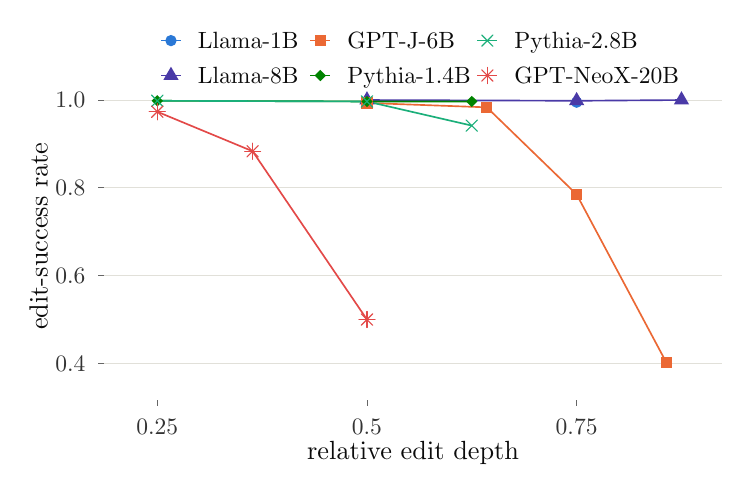
\begin{tikzpicture}[x=1pt,y=1pt]
\definecolor{fillColor}{RGB}{255,255,255}
\path[use as bounding box,fill=fillColor,fill opacity=0.00] (0,0) rectangle (252.94,158.99);
\begin{scope}
\path[clip] (  0.00,  0.00) rectangle (252.94,158.99);
\definecolor{fillColor}{RGB}{255,255,255}

\path[fill=fillColor] (  0.00, -0.00) rectangle (252.94,158.99);
\end{scope}
\begin{scope}
\path[clip] ( 27.59, 24.34) rectangle (250.95,143.00);
\definecolor{drawColor}{RGB}{225,224,217}

\path[draw=drawColor,line width= 0.3pt,line join=round] ( 27.59, 37.66) --
	(250.95, 37.66);

\path[draw=drawColor,line width= 0.3pt,line join=round] ( 27.59, 69.39) --
	(250.95, 69.39);

\path[draw=drawColor,line width= 0.3pt,line join=round] ( 27.59,101.12) --
	(250.95,101.12);

\path[draw=drawColor,line width= 0.3pt,line join=round] ( 27.59,132.84) --
	(250.95,132.84);
\definecolor{drawColor}{RGB}{74,58,167}

\path[draw=drawColor,line width= 0.6pt,line join=round] (122.60,132.84) --
	(198.36,132.57) --
	(236.25,132.84);
\definecolor{drawColor}{RGB}{235,104,52}

\path[draw=drawColor,line width= 0.6pt,line join=round] (122.60,131.78) --
	(165.91,130.20) --
	(198.36, 98.74) --
	(230.82, 37.93);
\definecolor{drawColor}{RGB}{0,131,0}

\path[draw=drawColor,line width= 0.6pt,line join=round] ( 46.84,132.57) --
	(122.60,132.32) --
	(160.48,132.32);
\definecolor{drawColor}{RGB}{27,175,122}

\path[draw=drawColor,line width= 0.6pt,line join=round] ( 46.84,132.57) --
	(122.60,132.32) --
	(160.48,123.60);
\definecolor{drawColor}{RGB}{227,73,72}

\path[draw=drawColor,line width= 0.6pt,line join=round] ( 46.84,128.61) --
	( 81.27,114.34) --
	(122.60, 53.53);
\definecolor{fillColor}{RGB}{42,120,214}

\path[fill=fillColor] (198.36,132.05) circle (  2.05);
\definecolor{fillColor}{RGB}{74,58,167}

\path[fill=fillColor] (122.60,136.04) --
	(125.36,131.25) --
	(119.83,131.25) --
	cycle;

\path[fill=fillColor] (198.36,135.77) --
	(201.13,130.98) --
	(195.60,130.98) --
	cycle;

\path[fill=fillColor] (236.25,136.04) --
	(239.01,131.25) --
	(233.48,131.25) --
	cycle;
\definecolor{fillColor}{RGB}{235,104,52}

\path[fill=fillColor] (120.55,129.73) --
	(124.65,129.73) --
	(124.65,133.83) --
	(120.55,133.83) --
	cycle;

\path[fill=fillColor] (163.85,128.14) --
	(167.96,128.14) --
	(167.96,132.25) --
	(163.85,132.25) --
	cycle;

\path[fill=fillColor] (196.31, 96.69) --
	(200.42, 96.69) --
	(200.42,100.79) --
	(196.31,100.79) --
	cycle;

\path[fill=fillColor] (228.77, 35.88) --
	(232.87, 35.88) --
	(232.87, 39.99) --
	(228.77, 39.99) --
	cycle;
\definecolor{fillColor}{RGB}{0,131,0}

\path[fill=fillColor] ( 44.78,132.57) --
	( 46.84,134.63) --
	( 48.89,132.57) --
	( 46.84,130.52) --
	cycle;

\path[fill=fillColor] (120.55,132.32) --
	(122.60,134.37) --
	(124.65,132.32) --
	(122.60,130.27) --
	cycle;

\path[fill=fillColor] (158.43,132.32) --
	(160.48,134.37) --
	(162.54,132.32) --
	(160.48,130.27) --
	cycle;
\definecolor{drawColor}{RGB}{27,175,122}

\path[draw=drawColor,line width= 0.4pt,line join=round,line cap=round] ( 44.78,130.52) -- ( 48.89,134.63);

\path[draw=drawColor,line width= 0.4pt,line join=round,line cap=round] ( 44.78,134.63) -- ( 48.89,130.52);

\path[draw=drawColor,line width= 0.4pt,line join=round,line cap=round] (120.55,130.27) -- (124.65,134.37);

\path[draw=drawColor,line width= 0.4pt,line join=round,line cap=round] (120.55,134.37) -- (124.65,130.27);

\path[draw=drawColor,line width= 0.4pt,line join=round,line cap=round] (158.43,121.54) -- (162.54,125.65);

\path[draw=drawColor,line width= 0.4pt,line join=round,line cap=round] (158.43,125.65) -- (162.54,121.54);
\definecolor{drawColor}{RGB}{227,73,72}

\path[draw=drawColor,line width= 0.4pt,line join=round,line cap=round] ( 44.78,126.56) -- ( 48.89,130.67);

\path[draw=drawColor,line width= 0.4pt,line join=round,line cap=round] ( 44.78,130.67) -- ( 48.89,126.56);

\path[draw=drawColor,line width= 0.4pt,line join=round,line cap=round] ( 43.93,128.61) -- ( 49.74,128.61);

\path[draw=drawColor,line width= 0.4pt,line join=round,line cap=round] ( 46.84,125.71) -- ( 46.84,131.52);

\path[draw=drawColor,line width= 0.4pt,line join=round,line cap=round] ( 79.22,112.28) -- ( 83.33,116.39);

\path[draw=drawColor,line width= 0.4pt,line join=round,line cap=round] ( 79.22,116.39) -- ( 83.33,112.28);

\path[draw=drawColor,line width= 0.4pt,line join=round,line cap=round] ( 78.37,114.34) -- ( 84.18,114.34);

\path[draw=drawColor,line width= 0.4pt,line join=round,line cap=round] ( 81.27,111.43) -- ( 81.27,117.24);

\path[draw=drawColor,line width= 0.4pt,line join=round,line cap=round] (120.55, 51.47) -- (124.65, 55.58);

\path[draw=drawColor,line width= 0.4pt,line join=round,line cap=round] (120.55, 55.58) -- (124.65, 51.47);

\path[draw=drawColor,line width= 0.4pt,line join=round,line cap=round] (119.70, 53.53) -- (125.50, 53.53);

\path[draw=drawColor,line width= 0.4pt,line join=round,line cap=round] (122.60, 50.62) -- (122.60, 56.43);
\end{scope}
\begin{scope}
\path[clip] (  0.00,  0.00) rectangle (252.94,158.99);
\definecolor{drawColor}{gray}{0.20}

\node[text=drawColor,anchor=base east,inner sep=0pt, outer sep=0pt, scale=  0.85] at ( 20.87, 34.90) {0.4};

\node[text=drawColor,anchor=base east,inner sep=0pt, outer sep=0pt, scale=  0.85] at ( 20.87, 66.62) {0.6};

\node[text=drawColor,anchor=base east,inner sep=0pt, outer sep=0pt, scale=  0.85] at ( 20.87, 98.35) {0.8};

\node[text=drawColor,anchor=base east,inner sep=0pt, outer sep=0pt, scale=  0.85] at ( 20.87,130.08) {1.0};
\end{scope}
\begin{scope}
\path[clip] (  0.00,  0.00) rectangle (252.94,158.99);
\definecolor{drawColor}{gray}{0.40}

\path[draw=drawColor,line width= 0.3pt,line join=round] ( 25.59, 37.66) --
	( 27.59, 37.66);

\path[draw=drawColor,line width= 0.3pt,line join=round] ( 25.59, 69.39) --
	( 27.59, 69.39);

\path[draw=drawColor,line width= 0.3pt,line join=round] ( 25.59,101.12) --
	( 27.59,101.12);

\path[draw=drawColor,line width= 0.3pt,line join=round] ( 25.59,132.84) --
	( 27.59,132.84);
\end{scope}
\begin{scope}
\path[clip] (  0.00,  0.00) rectangle (252.94,158.99);
\definecolor{drawColor}{gray}{0.40}

\path[draw=drawColor,line width= 0.3pt,line join=round] ( 46.84, 22.34) --
	( 46.84, 24.34);

\path[draw=drawColor,line width= 0.3pt,line join=round] (122.60, 22.34) --
	(122.60, 24.34);

\path[draw=drawColor,line width= 0.3pt,line join=round] (198.36, 22.34) --
	(198.36, 24.34);
\end{scope}
\begin{scope}
\path[clip] (  0.00,  0.00) rectangle (252.94,158.99);
\definecolor{drawColor}{gray}{0.20}

\node[text=drawColor,anchor=base,inner sep=0pt, outer sep=0pt, scale=  0.85] at ( 46.84, 12.08) {0.25};

\node[text=drawColor,anchor=base,inner sep=0pt, outer sep=0pt, scale=  0.85] at (122.60, 12.08) {0.5};

\node[text=drawColor,anchor=base,inner sep=0pt, outer sep=0pt, scale=  0.85] at (198.36, 12.08) {0.75};
\end{scope}
\begin{scope}
\path[clip] (  0.00,  0.00) rectangle (252.94,158.99);
\definecolor{drawColor}{RGB}{11,11,11}

\node[text=drawColor,anchor=base,inner sep=0pt, outer sep=0pt, scale=  0.95] at (139.27,  3.06) {relative edit depth};
\end{scope}
\begin{scope}
\path[clip] (  0.00,  0.00) rectangle (252.94,158.99);
\definecolor{drawColor}{RGB}{11,11,11}

\node[text=drawColor,rotate= 90.00,anchor=base,inner sep=0pt, outer sep=0pt, scale=  0.95] at (  7.18, 83.67) {edit-success rate};
\end{scope}
\begin{scope}
\path[clip] (  0.00,  0.00) rectangle (252.94,158.99);
\definecolor{drawColor}{RGB}{42,120,214}

\path[draw=drawColor,line width= 0.6pt,line join=round] ( 48.18,154.31) -- ( 55.38,154.31);
\definecolor{fillColor}{RGB}{42,120,214}

\path[fill=fillColor] ( 51.78,154.31) circle (  2.05);
\end{scope}
\begin{scope}
\path[clip] (  0.00,  0.00) rectangle (252.94,158.99);
\definecolor{drawColor}{RGB}{74,58,167}

\path[draw=drawColor,line width= 0.6pt,line join=round] ( 48.18,141.68) -- ( 55.38,141.68);
\definecolor{fillColor}{RGB}{74,58,167}

\path[fill=fillColor] ( 51.78,144.88) --
	( 54.55,140.09) --
	( 49.02,140.09) --
	cycle;
\end{scope}
\begin{scope}
\path[clip] (  0.00,  0.00) rectangle (252.94,158.99);
\definecolor{drawColor}{RGB}{235,104,52}

\path[draw=drawColor,line width= 0.6pt,line join=round] (102.15,154.31) -- (109.35,154.31);
\definecolor{fillColor}{RGB}{235,104,52}

\path[fill=fillColor] (103.70,152.25) --
	(107.80,152.25) --
	(107.80,156.36) --
	(103.70,156.36) --
	cycle;
\end{scope}
\begin{scope}
\path[clip] (  0.00,  0.00) rectangle (252.94,158.99);
\definecolor{drawColor}{RGB}{0,131,0}

\path[draw=drawColor,line width= 0.6pt,line join=round] (102.15,141.68) -- (109.35,141.68);
\definecolor{fillColor}{RGB}{0,131,0}

\path[fill=fillColor] (103.70,141.68) --
	(105.75,143.74) --
	(107.80,141.68) --
	(105.75,139.63) --
	cycle;
\end{scope}
\begin{scope}
\path[clip] (  0.00,  0.00) rectangle (252.94,158.99);
\definecolor{drawColor}{RGB}{27,175,122}

\path[draw=drawColor,line width= 0.6pt,line join=round] (162.50,154.31) -- (169.70,154.31);

\path[draw=drawColor,line width= 0.4pt,line join=round,line cap=round] (164.05,152.25) -- (168.15,156.36);

\path[draw=drawColor,line width= 0.4pt,line join=round,line cap=round] (164.05,156.36) -- (168.15,152.25);
\end{scope}
\begin{scope}
\path[clip] (  0.00,  0.00) rectangle (252.94,158.99);
\definecolor{drawColor}{RGB}{227,73,72}

\path[draw=drawColor,line width= 0.6pt,line join=round] (162.50,141.68) -- (169.70,141.68);

\path[draw=drawColor,line width= 0.4pt,line join=round,line cap=round] (164.05,139.63) -- (168.15,143.74);

\path[draw=drawColor,line width= 0.4pt,line join=round,line cap=round] (164.05,143.74) -- (168.15,139.63);

\path[draw=drawColor,line width= 0.4pt,line join=round,line cap=round] (163.20,141.68) -- (169.00,141.68);

\path[draw=drawColor,line width= 0.4pt,line join=round,line cap=round] (166.10,138.78) -- (166.10,144.59);
\end{scope}
\begin{scope}
\path[clip] (  0.00,  0.00) rectangle (252.94,158.99);
\definecolor{drawColor}{RGB}{11,11,11}

\node[text=drawColor,anchor=base west,inner sep=0pt, outer sep=0pt, scale=  0.85] at ( 61.53,151.54) {Llama-1B};
\end{scope}
\begin{scope}
\path[clip] (  0.00,  0.00) rectangle (252.94,158.99);
\definecolor{drawColor}{RGB}{11,11,11}

\node[text=drawColor,anchor=base west,inner sep=0pt, outer sep=0pt, scale=  0.85] at ( 61.53,138.92) {Llama-8B};
\end{scope}
\begin{scope}
\path[clip] (  0.00,  0.00) rectangle (252.94,158.99);
\definecolor{drawColor}{RGB}{11,11,11}

\node[text=drawColor,anchor=base west,inner sep=0pt, outer sep=0pt, scale=  0.85] at (115.50,151.54) {GPT-J-6B};
\end{scope}
\begin{scope}
\path[clip] (  0.00,  0.00) rectangle (252.94,158.99);
\definecolor{drawColor}{RGB}{11,11,11}

\node[text=drawColor,anchor=base west,inner sep=0pt, outer sep=0pt, scale=  0.85] at (115.50,138.92) {Pythia-1.4B};
\end{scope}
\begin{scope}
\path[clip] (  0.00,  0.00) rectangle (252.94,158.99);
\definecolor{drawColor}{RGB}{11,11,11}

\node[text=drawColor,anchor=base west,inner sep=0pt, outer sep=0pt, scale=  0.85] at (175.85,151.54) {Pythia-2.8B};
\end{scope}
\begin{scope}
\path[clip] (  0.00,  0.00) rectangle (252.94,158.99);
\definecolor{drawColor}{RGB}{11,11,11}

\node[text=drawColor,anchor=base west,inner sep=0pt, outer sep=0pt, scale=  0.85] at (175.85,138.92) {GPT-NeoX-20B};
\end{scope}
\end{tikzpicture}
